\paragraph{QuizziPedia::Front-End::Views::QuestionsManagementView}
\begin{figure} [ht]
	\centering
	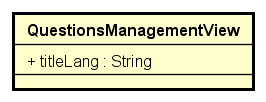
\includegraphics[scale=0.80]{UML/Classi/Front-End/QuizziPedia_Front-end_Views_QuestionsManagementView.png}
	\caption{QuizziPedia::Front-End::Views::QuestionsManagementView}
\end{figure} \FloatBarrier
\begin{itemize}
	\item \textbf{Descrizione}: view contenente l'elenco delle domande create; 
	\item \textbf{Utilizzo}: visualizza l'elenco delle domande create permettendo all'utente di crearne una nuova o di modificarne una presente nell'elenco;
	\item \textbf{Relazioni con altre classi}:
	\begin{itemize} 
		\item \textit{IN} \texttt{QuestionsManagementModelView}: classe di tipo modelview la cui istanzazione è contenuta all'interno della variabile di ambiente \$scope di \texttt{Angular.js}. All'interno di essa sono presenti le variabili e i metodi necessari per il \textit{Two-Way Data-Binding\ped{G}} tra la view \texttt{QuestionsManagementView} e il controller \texttt{QuestionsManagementController};
		\item \textit{IN} \texttt{OneQuestionDirective}: rappresenta il componente grafico che visualizza all'utente l'anteprima della domanda che ha creato. Eseguendo l'azione di click su di essa sarà possibile modificare tale domanda. All'interno di \texttt{QuestionsManagementsView} verranno stampati a video tanti componenti quanti presenti nello \texttt{\$scope} isolato ad esso associato;
		\item \textit{IN} \texttt{NewQuestionButtonDirective}:  rappresenta il componente grafico che permette all'utente di posizionarsi nella view di creazione di una nuova domanda;
		\item \textit{IN} \texttt{LangModel}: rappresenta il modello delle informazioni per la giusta traduzione dell'applicazione. 
	\end{itemize}
	\item \textbf{Attributi}:
	\begin{itemize}
		\item \texttt{+ titleLangQuestionsManagement: String} \\ Attributo che viene utilizzato per visualizzare la giusta traduzione del titolo della pagina, in italiano o in inglese.
	\end{itemize}
\end{itemize}
